%!TEX root = ../template.tex
%%%%%%%%%%%%%%%%%%%%%%%%%%%%%%%%%%%%%%%%%%%%%%%%%%%%%%%%%%%%%%%%%%%%
%% chapter5.tex
%% NOVA thesis document file
%%
%% Chapter with lots of dummy text
%%%%%%%%%%%%%%%%%%%%%%%%%%%%%%%%%%%%%%%%%%%%%%%%%%%%%%%%%%%%%%%%%%%%

\typeout{NT FILE chapter5.tex}%

\chapter{Work Plan}
\label{cha:work_plan}


\begin{itemize}
    \item \textbf{Mockup Design}
    \item \textbf{Database Creation for Repository}: Start with the structure for one object
    \item \textbf{GIS Implementation and Manipulation}
    \item \textbf{Integrate GIS Map in Unity}
    \item \textbf{VR Integration}: Artifacts interaction with 3D models/reconstruction – Start with the manipulation of one object, including layers interaction
    \item \textbf{Implementation of AR Functionalities}
\end{itemize}

\begin{figure}[h!]
    \centering
    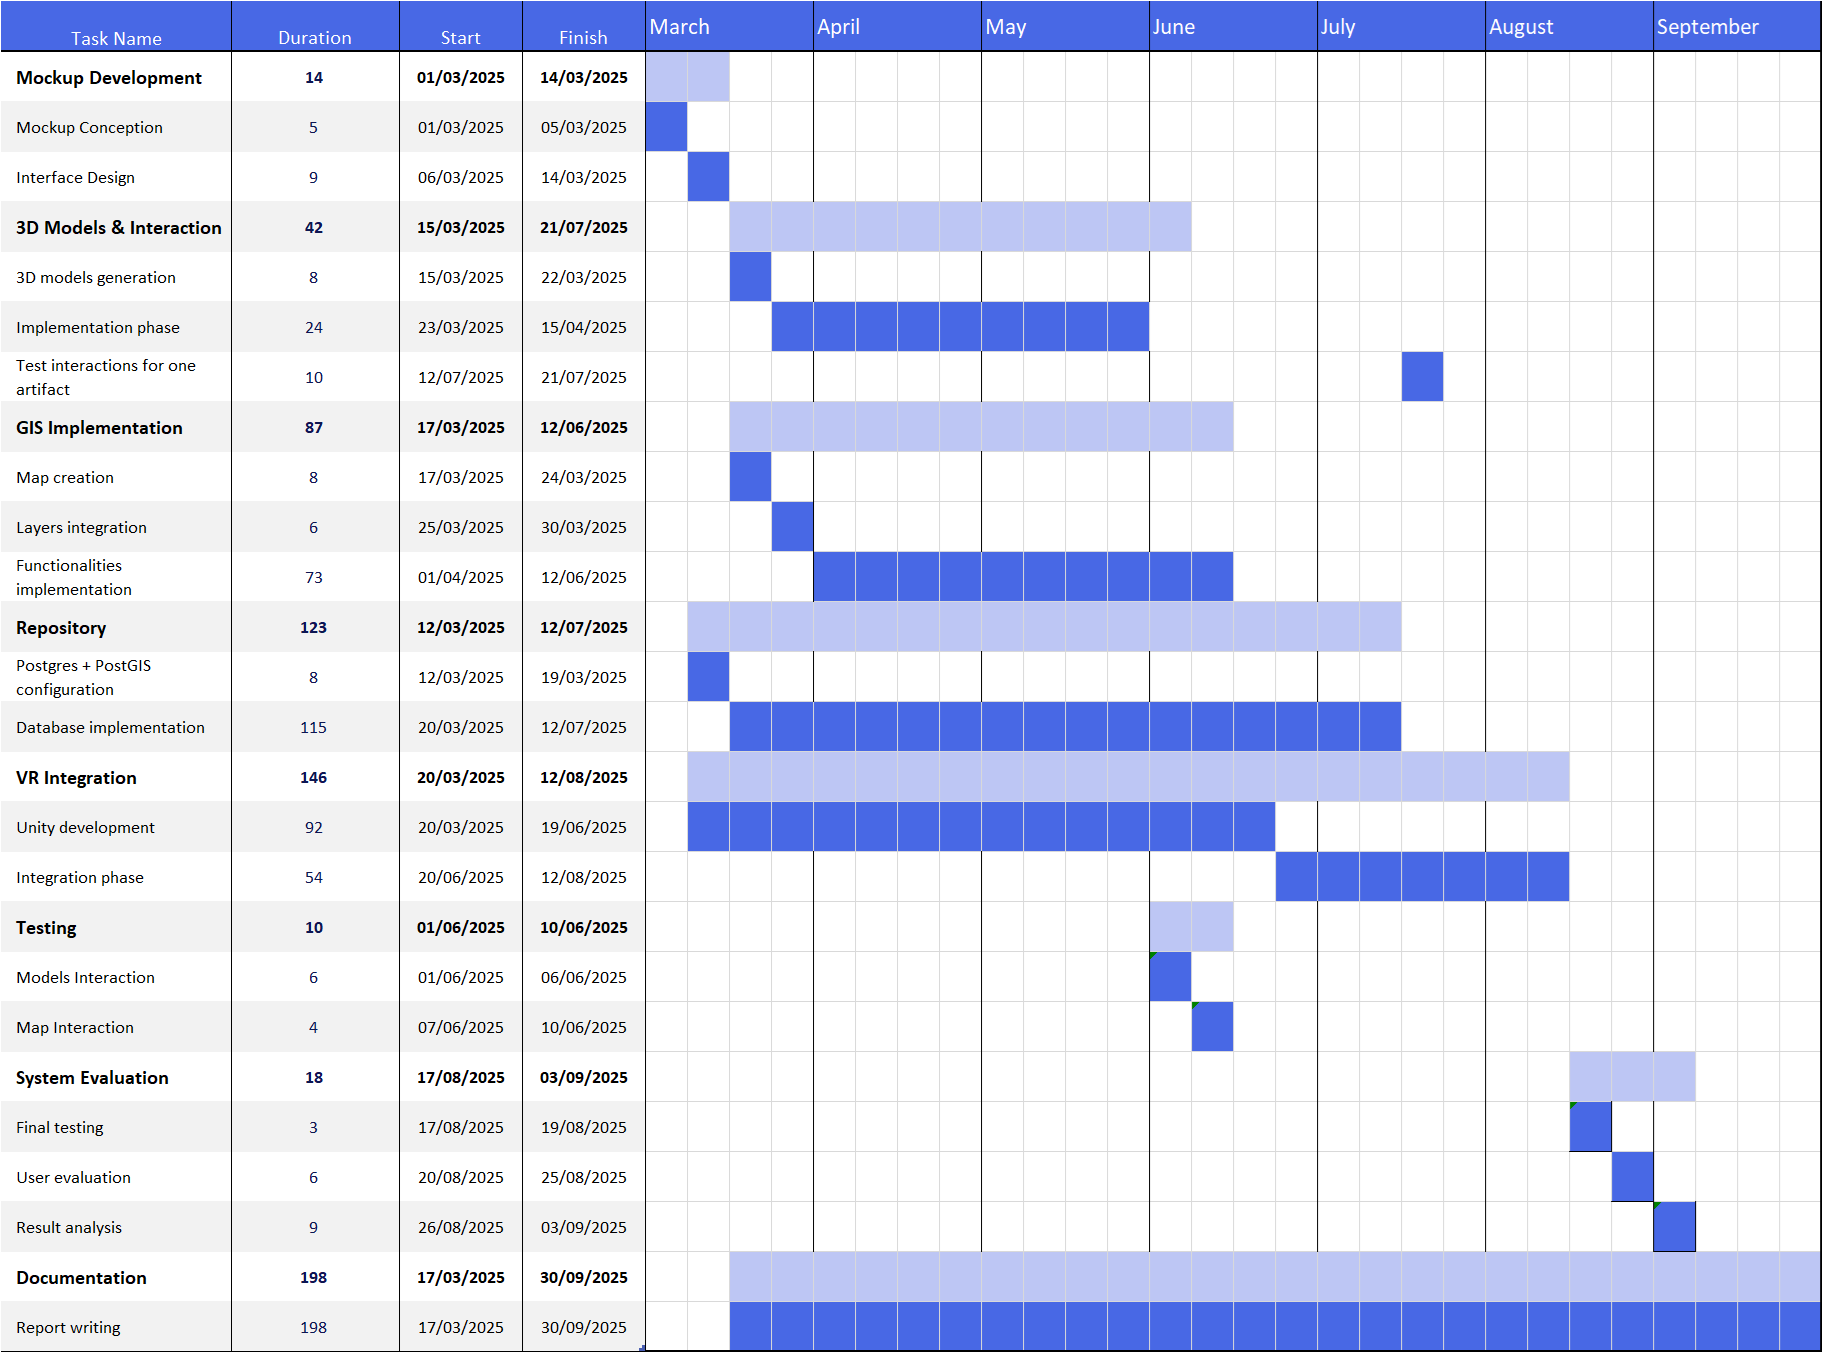
\includegraphics[width=1.0\linewidth]{Gantt_chart}
    \caption{Gantt Chart Representation of the Work Plan.}
    \label{fig:gantt_chart}
  \end{figure}
  \FloatBarrier